\section{RASim}
\label{rasim:rasim}
El simulador \ac{RASim} proporciona un entorno de trabajo para el entrenamiento de la \ac{RA}. En esta tesis se ha trabajado junto con los demás participantes de \ac{RASimAs} para realizar una mesa de trabajo que permite al usuario sentirse inmerso dentro de un entorno que sea lo más parecido a la situación real que se encontrarán en su futuro profesional.

El simulador consta de un maniquí que permitirá al usuario interaccionar físicamente acompañado de unos dispositivos que simulan una sonda de ultrasonidos y una aguja. Estos dispositivos están conectados a un computador que es el sistema principal, dónde a través de dos monitores se mostrará al usuario información visual y a través de un dispositivo háptico se proporcionará respuesta táctil. Además, se incorporará un \ac{Courseware}\footnote{Término ampliamente utilizado en la industria } que servirá para proporcionar una plataforma de aprendizaje y al mismo tiempo poder recopilar métricas y mostrar información útil al usuario. Esta aplicación será la encargada de cargar diferentes escenarios, guardar sesiones de entrenamiento, mostrar tareas y lecciones específicas de entrenamiento.
El prototipo creado tendrá que ser evaluado como parte del proyecto europeo en estudios clínicos controlados dirigidos tanto a expertos como estudiantes de anestesiología. Antes de alcanzar los experimentos clínicos, cada módulo del simulador debe ser probado por separado (\ac{WP}4 sección \ref{art:rasimas}) para asegurar el proceso de evaluación y permitir un desarrollo iterativo con el objetivo de construir un prototipo validado y fiable (\ac{WP}5 sección \ref{art:rasimas}). Para cumplir con ello se han propuesto las siguientes especificaciones para el simulador:

\begin{itemize}
    \item Computador: el sistema donde se ejecutará el sistema deberá ser lo suficiente potente como para ejecutar simulaciones físicas que permiten simular el comportamiento de los tejidos, retroalimentación háptica y representación visual.
    \item Plataforma de trabajo: para estandarizar el entorno de trabajo se ha diseñado una plataforma que permite conocer la disposición tanto del maniquí como de los dispositivos hápticos con el objetivo de ser fácilmente reproducible en diferentes instituciones. Deberá estar diseñado para personas diestras y zurdas.
    \item Maniquí y región de interés: con el objetivo de proporcionar el mayor realismo posible, se ha propuesto incluir un maniquí en la plataforma para que el usuario se sienta más inmerso y el entrenamiento sea más efectivo.
    \item Monitores: es necesario mostrar información visual sobre la habitación virtual y la imagen de \ac{US}. Además, se mostrará información útil para el aprendizaje.
    \item Sonda de ultrasonidos: es uno de los instrumentos principales de la \ac{RA}, por ello conviene que la sonda sea lo más realista posible.
    \item Aguja: instrumento fundamental en el procedimiento. Al ser una parte importante del entrenamiento, el simulador captura su movimiento y posición y devuelve fuerzas que simularan las sensaciones para el usuario como si fuera en un entorno real.
    \item \ac{Courseware}: una aplicación que permita integrar todos los elementos del sistema además de proporcionar un sistema de entrenamiento y evaluación.
\end{itemize}

La responsabilidad del primer prototipo de \ac{RASim} recae en el equipo de trabajo de \ac{SG}, siendo cada módulo desarrollado por diferentes integrantes del proyecto. Aun así, la comunicación entre los diferentes grupos ha sido fundamental para conseguir una buena cohesión de todos los elementos del simulador. El autor de esta tesis ha sido el encargado de desarrollar el \ac{Courseware} pero ha estado colaborando activamente en el desarrollo y puesta en funcionamiento del prototipo, realizando contribuciones en la mayoría de los módulos.


\subsection{Caso de uso}
\label{rasim:casodeusorasim}

El simulador está orientado para entrenar el procedimiento de \ac{RA} de manera que proporcione una evaluación sumativa al supervisar el progreso del alumno. Por ello el usuario, normalmente estudiante de anestesiología, tiene designado un tiempo y objetivos mínimos que deberá cumplir. El usuario se sentará delante del entorno de trabajo y el primer paso será identificarse en el sistema para poder almacenar y seguir su evolución durante todo el proceso. En las primeras sesiones, el usuario podrá revisar contenido multimedia para familiarizarse con el simulador y el procedimiento que se requiera entrenar. El siguiente paso, será realizar una sesión guiada en la cual consiste en que el simulador va orientando al usuario en todos los pasos que debe realizar para completar con éxito el procedimiento médico. Cada sesión realizada, el simulador mostrará una retroalimentación sobre el desempeño del usuario en esa sesión, métricas recogidas por el simulador y una información asociada.
Una vez completada la primera sesión guiada, el usuario podrá repetir la sesión guiada o realizar una sesión libre, en la que el simulador no proporcionará ninguna indicación y sólo se recogerán métricas de la sesión. Estos valores serán enviados a un servidor dónde el supervisor podrá consultar y revisar la evolución de los usuarios.


\subsection{Arquitectura del simulador}
\label{rasim:arqrasim}
Siguiendo la arquitectura de un simulador de \ac{RV} tipo que se puede observar en la figura \ref{fig:RVarq}  en el capítulo \ref{art:simulador}, un simulador puede ser definido por una serie de componentes. Los dispositivos de entrada y salida se comunican con un motor de \ac{RV} que calcula todas simulaciones físicas y visuales según la escena virtual o entorno de aprendizaje con el que haya sido programado. A continuación se procede a explicar cada componente por separado. 

\subsubsection{Motor de \ac{RV}}

Uno de los componentes principales de un simulador de \ac{RV} es el motor donde se producen todos los cálculos que permiten simular la escena virtual. 
En el contexto de \ac{RASim}, es lógico que este simulador tenga un núcleo que realiza las simulaciones físicas y cálculos necesarios con el objetivo de comunicarse con los dispositivos de entrada y salida. Además, también es necesario un núcleo de simulación que proporcione las imágenes de \ac{US} para conseguir mostrar una simulación realista que pueda ayudar al usuario. Por último, el sistema también deberá \emph{renderizar} la escena con la información de los dispositivos para ayudar al usuario a que alcance mayor inmersión de la escena. 

Debido a que el proyecto \ac{RASimAs} participan multitud de instituciones, los módulos encargados de cada tarea han sido desarrollado independientemente por cada participante y se presentarán en los siguientes párrafos.

\paragraph{Simulación visual}\mbox{}\\

\emph{H3D}\cite{asdf} es una librería de código abierto (\ac{GPL})  orientada a la utilización de hápticos en entornos 3D desarrollado por la empresa \emph{Sensegraphics}. 

\emph{H3D} sirve como punto de comunicación entre el software y los dispositivos.También es el encargado de recopilar la información de los dispositivos de entrada.
En cuanto el simulador es iniciado, \emph{H3D} se encarga de cargar la escena seleccionada utilizando el formato \ac{X3D}, e inicia el módulo de simulación física, y activa los dispositivos, tanto el dispositivo háptico, como el dispositivo de seguimiento. La vista del paciente y la sala de operaciones es \emph{renderizada} por \emph{H3D} a través de su gestor de ventanas. Las simulaciones físicas y el cálculo de las deformaciones de los tejidos como consecuencia de la colisión de los instrumentos médicos serán calculadas en el siguiente componte del simulador.

\paragraph{Simulación física}\mbox{}\\

En esta ocasión, es el software \emph{SOFA} desarrollado por el grupo \ac{INRIA} el encargado de realizar las simulaciones físicas. Esto permite simular la deformación de los tejidos al contacto de la sonda o la aguja, además de proporcionar la respuesta física a la aguja que será retransmitida al dispositivo háptico.

La librería \emph{SOFA} es código abierto (bajo licencia \ac{LGPL}) y dispone de multitud de métodos y algoritmos matemáticos usados en simulación como distintos \emph{solvers}\footnote{herramienta matemática para resolver sistemas de ecuaciones lineales}, modelos físicos como \ac{FEM}, detección de colisiones, simulación de tejidos rígidos o flexibles.

En \ac{RASim}, \emph{SOFA} realiza las siguientes tareas:
\begin{itemize}
    \item Deformación de la piel y otros tejidos producida por la interacción de los instrumentos médicos utilizando el método \ac{FEM} co-rotacional.
    \item La interacción con la aguja a través de diferentes tipos de tejidos, simulando la penetración de la piel y las fascias, además de la fricción de los demás tejidos.
   \item La contracción de los músculos con una respuesta física según sus propiedades mecánicas.
    
\end{itemize}

\paragraph{Simulación de ultrasonidos} \mbox{}\\

En cuanto a la simulación de la imagen de ultrasonidos, se utiliza una librería basada en \ac{ViSTA} desarrollado por el grupo \ac{RWTH}. \ac{ViSTA} es código abierto (bajo licencia \ac{LGPL}) y se utiliza para implementar el algoritmo con el que se simula la generación de imágenes de \ac{US}.

El módulo de ultrasonidos está desarrollado con un algoritmo basado en métodos acústicos geométricos \cite{Law2015}, el cual es clasificado como un enfoque \emph{generativo}. Pensando geométricamente, la onda de sonidos se puede aproximar a través de rayos que interaccionan con elementos de la escena, por consiguiente producen un reflejo del rayo refractado o dispersado. Estos rayos se definen por energía acústica, que puede ser absorbida o disipada durante la interacción con la escena. Esta energía es usada para calcular la intensidad de los ecos y en consecuencia la intensidad de los \emph{píxeles} que servirán para construir la imagen resultante.

Para alcanzar tiempos interactivos en presentar las imágenes de ultrasonidos, la mayor parte de los intensos cálculos y operaciones pesadas son realizadas durante un proceso previo. Específicamente, en esta etapa se generan un campo acústico que defina las propiedades del haz de la sonda y el transductor, las texturas tridimensionales que serán usadas para simular la dispersión del rayo y adicionalmente las estructuras de datos auxiliares que ayudarán a acelerar el proceso de simulación.
Así, de esta manera, cuando el objetivo es tener una respuesta interactiva, sólo es necesario la posición y orientación de la sonda virtual que se usará para calcular el origen y la dirección de los rayos acústicos. Estos rayos serán muestreados a través de la escena, estimando la energía reflejada y la distancia recorrida a través de los tejidos. Por otra parte, el remanente de energía transmitida, se tienen en cuenta absorciones y reflexiones es tenida en cuanta generar la imagen final.

\subsubsection{Dispositivos de entrada y salida}

Una característica importante de una herramienta de \ac{RV} es la inmersión del usuario en el sistema. Esta inmersión está normalmente muy influenciada por los dispositivos de entrada y salida que le conecta con el motor de \ac{RV}. Cuanto más se asemejen a la realidad, proporcionarán una sensación de inmersión y presencia que ayudará al usuario a mejorar su experiencia en el sistema y por tanto, el objetivo que hubiera detrás de éste (entrenamiento, preparación, etc...). Normalmente, como se ha introducido en el capítulo \ref{cap:intro}, estos dispositivos están orientados a determinados canales sensoriales. En este sistema, sólo se ha considerado el canal visual y el táctil debido a que el procedimiento de \ac{RA} no implica otro tipo de sentidos. A continuación, se hará una descripción de los dispositivos que componen el prototipo desarrollado en el proyecto.

\paragraph{Vistas del paciente y del ecógrafo}\mbox{}\\

La vista es el sentido de entrada dominante en muchos aspectos cotidianos y en este simulador, concretamente, es necesario que el usuario pueda situar los instrumentos médicos en relación con la anatomía del paciente. Además, necesita recabar toda la información posible de los tejidos internos que le proporciona la imagen de ultrasonidos y no puede observarse a simple vista. Por tanto, el usuario utiliza su capacidad visual para colocar los instrumentos médicos en la posición requerida y a la vez requiere del ecógrafo para su correcto desempeño.

Para representar la vista del paciente y de la máquina de ultrasonidos, se ha incorporado dos pantallas al entorno de trabajo del simulador. 
En uno de ellos se muestra la vista del paciente. Esta consiste en la \emph{renderización} de la escena virtual dónde se encuentra el modelo anatómico de un paciente y una representación virtual de los instrumentos médicos. Adicionalmente, esta vista se puede utilizar para añadir elementos virtuales que mejoren la efectividad del entrenamiento. 
Por otra parte, en el otro monitor se utiliza para mostrar el software de entrenamiento que incluye la imagen de ultrasonidos generada por el motor de \ac{RV}.

A continuación, se va a proceder a describir aquellos dispositivos que utilizan el canal táctil. \todo{este párrafo va bien aquí?}

\paragraph{Sonda de ultrasonidos}\mbox{}\\

El posicionamiento de la sonda de ultrasonidos es clave en el procedimiento de \ac{RA} debido a que es fundamental encontrar el nervio a anestesiar. Para simular este aparato médico se ha diseñado un modelo impreso en 3D que imita una sonda real que envuelve a un dispositivo de seguimiento. Para esta finalidad, se ha utilizado un \ac{tracker} magnético\footnote{ Ascension 3D-Guidance trakSTAR, módelo 800 \cite{Ascension}} como se puede observar en la figura \ref{fig:tracker}. 
Este dispositivo es capaz de saber la posición de un receptor o sensor gracias a la generación de un campo magnético producido por un emisor. La deformación del campo magnético producido por el receptor ayuda al dispositivo a conocer su posición y orientación. Este sensor es el que se introduce dentro del modelo impreso y sirve para saber la posición de la sonda respecto a la mesa de trabajo. De esta manera el usuario puede apreciar de la misma forma que uno real.

\begin{figure}[h]
    \centering
    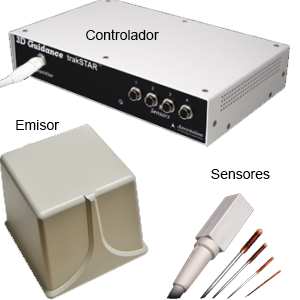
\includegraphics{IMG/tracker.png}
    \caption{\emph{Ascension 3D-Guidance trakSTAR, módelo 800} \cite{Ascension} utilizado en \ac{RASim}}
    \label{fig:tracker}
\end{figure}

En un principio, el diseño del modelo 3D intenta recrear la sonda original a la vez que se incluye el dispositivo de seguimiento dentro de él. Se ha diseñado un modelo compuesto por dos piezas que en el interior acoge el sensor sin que el usuario sea consciente (ver figura \ref{fig:m3d}). Además, el propio cable del sensor es similar al cable que se encontrarán los usuarios en un entorno real.

\begin{figure}[h]
    \centering
    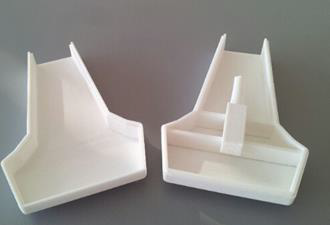
\includegraphics[width=0.5\textwidth]{IMG/modelo3d.png}
    \caption{Primer prototipo del modelo impreso de la sonda de ultrasonidos para alojar el sensor del \emph{tracker} magnético.}
    \label{fig:m3d}
\end{figure}

Debido a limitaciones de hardware de poder recrear fielmente la deformación de los tejidos de la piel cuando el médico presiona la sonda contra ella, se decidió junto con los profesionales médicos del proyecto que habría que incorporar algún mecanismo que ofreciera al usuario el realismo de la elasticidad de la piel. Así de esta manera, se ideó una pieza adicional conectada al modelo 3D a través de un muelle que permitía la sensación de tejido flexible al usuario como se puede observar en la figura \ref{fig:m3dv2}.

\begin{figure}[h]
    \centering
    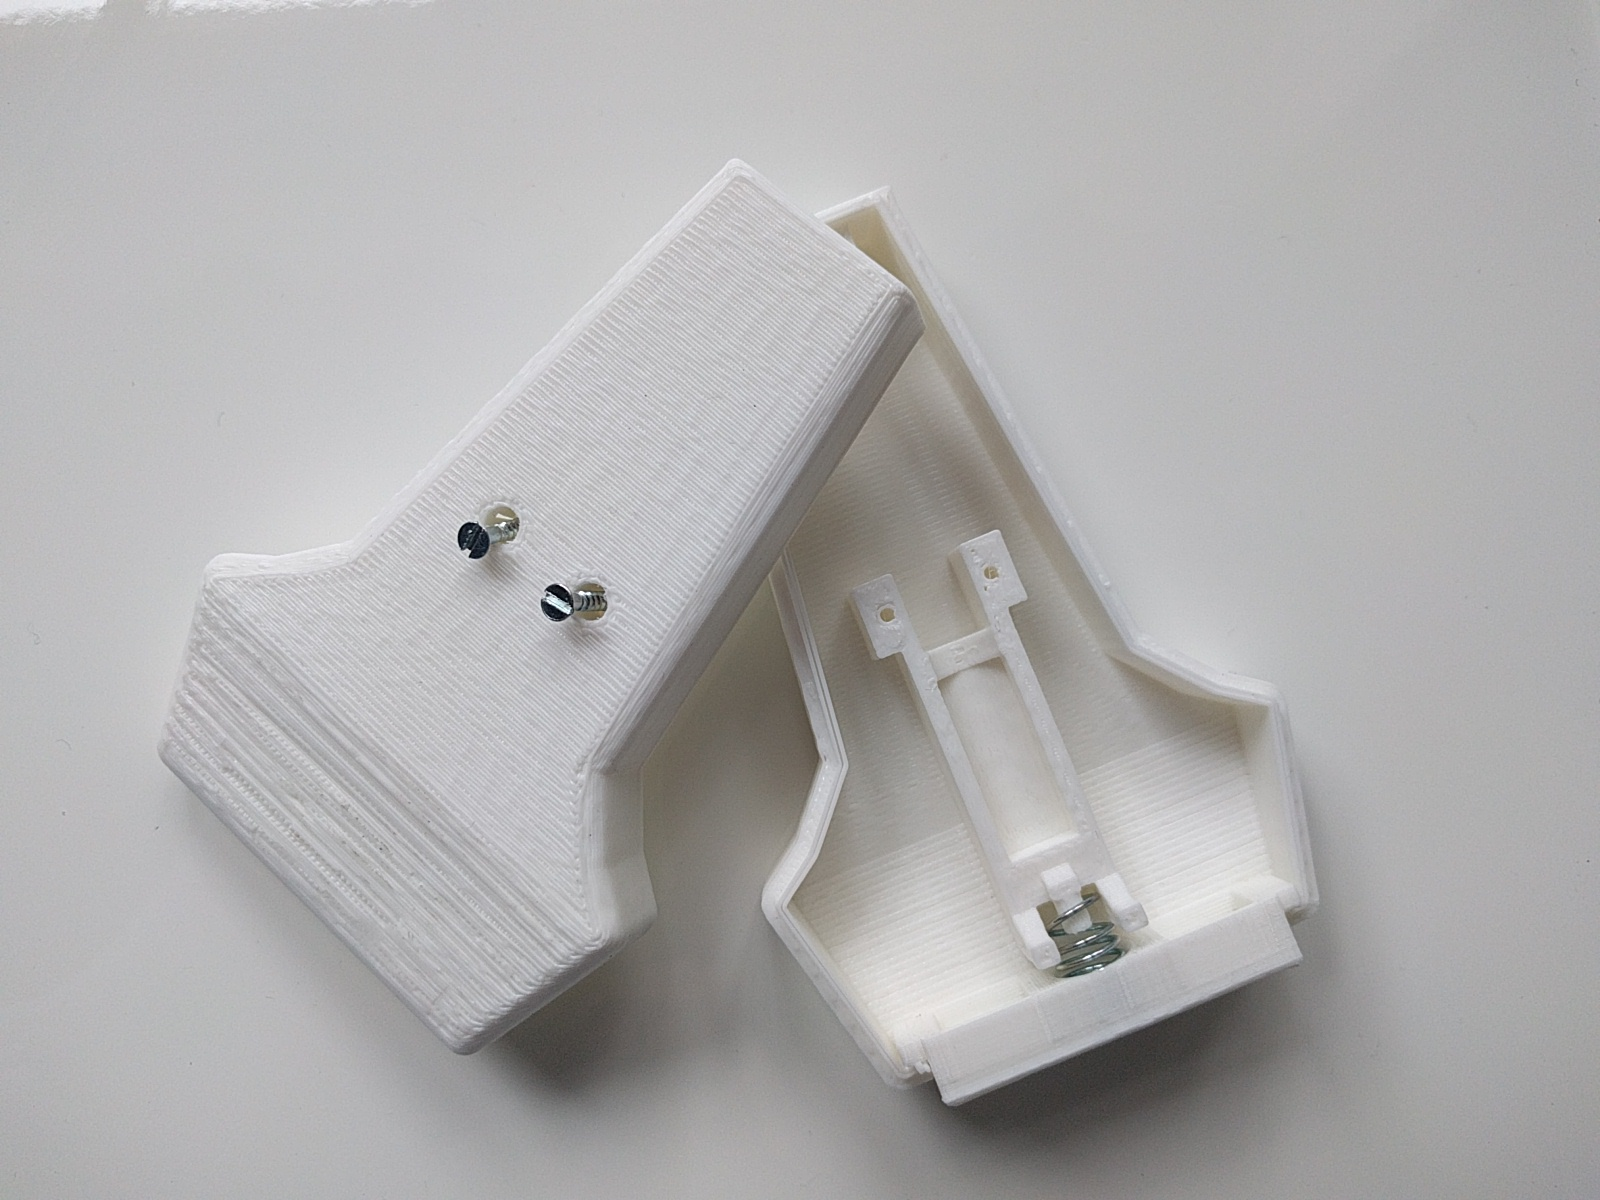
\includegraphics[width=0.5\textwidth]{IMG/modelo3dv2.jpg}
    \caption{Modelo impreso de la sonda de ultrasonidos con la actualización que permite sentir la elasticidad de la piel }
    \label{fig:m3dv2}
\end{figure}


\paragraph{Aguja}\mbox{}\\

Además de la localización del nervio, la inserción de la aguja y su aproximación al nervio que se va a anestesiar es un punto crucial del procedimiento de \ac{RA}. 

La inserción real de la aguja implica que su movimiento pueda definirse a través de 5 \ac{DOF}. La correcta posición, el movimiento adecuado y la sensación de la aguja es muy importante en el entrenamiento de los nuevos médicos. Por ello la selección del dispositivo con el que replicar estos comportamientos no es sencillo. Los \ac{tracker}s mágneticos anteriormente citados serían una buena solución debido a que son capaces de registrar el movimiento del sensor en sus 6 \ac{DOF}, pero estos dispositivos no están pensados para devolver retroalimentación al usuario. Los dispositivos hápticos suelen resolver este tipo de problema al ser utilizados como dispositivos de seguimiento y a la vez son capaces de reproducir fuerzas e interaccionar con el usuario.

Desde el proyecto \ac{RASimAs} se ha seleccionado el dispositivo \emph{Touch} de la empresa \emph{3D System}\cite{asdf}. Aunque este dispositivo solo es capaz de proporcionar fuerzas en los 3 \ac{DOF} básicos(x,y,z), hay que alcanzar un compromiso entre versatilidad y el presupuesto. Existen dispositivos hápticos que pueden ofrecer la experiencia de simular la inserción de una aguja, pero su complejidad implicaría un coste inasequible para la comercialización de un simulador y aumentaría la dificultad de una inmersión del usuario debido a que no existe dispositivo háptico con esas características de pequeñas dimensiones. Sin embargo, el dispositivo \emph{Touch} proporciona la posibilidad de que el sistema sea más barato y consiga cierto realismo. 
El usuario maneja este dispositivo a través de una especie de bolígrafo (\emph{stylus}) que es capaz de reconocer la posición, orientación y devolver fuerzas. Incluso es lo suficiente ligero para poder permitir su colocación en otras posiciones con el objetivo de permitir a los usuarios elegir con que mano utilizar los dispositivos.

Aun así, la utilización de este dispositivo para simular una aguja no esta exento de problemas. El objetivo es simular una aguja real pero el actuador del dispositivo es completamente diferente y sería muy difícil replicar el mismo comportamiento que se experimenta en una situación real.
Con el objetivo de solventar este problema, se ha intentado adaptar el bolígrafo que dispone para que aloje una aguja real utilizado en el procedimiento.
El dispositivo \emph{Touch} permite desmontar la punta del actuador con la intención de permitir a otros desarrolladores encajar nuevas creaciones a través de un conector tipo \emph{Jack}. En este caso, desde \ac{SG} se diseñó un modelo 3d que encaje en el conector de manera que la aguja pueda ser agarrada por el usuario. Esto permite que se puedan utilizar el mismo tipo de aguja estandarizando la solución como se puede ver en la figura \ref{fig:needle}.

\begin{figure}[h]
    \centering
    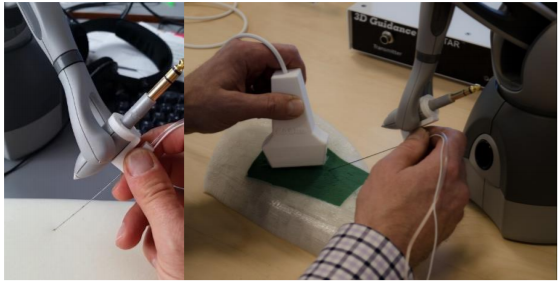
\includegraphics[width=0.5\textwidth]{IMG/needle.PNG}
    \caption{Primer prototipo para adjuntar una aguja real al dispositivo háptico.}
    \label{fig:needle}
\end{figure}

Esta solución, aunque bien diseñada, en las primeras pruebas mostró varios factores que hicieron descartarla por parte del comité médico. El desplazamiento entre el centro del conector del dispositivo háptico y el lugar donde el usuario agarraba la aguja junto con la flexibilidad de esta, introducía un desplazamiento virtual que hacía que el simulador no representará fielmente la posición real en el mundo virtual. Desde la \ac{URJC}, se sugirió una adaptación  anteriormente utilizada en un desarrollo anterior\cite{phantompen}. Esta versión encajaba en la forma de bolígrafo que tenía el dispositivo y permitía el uso de una aguja estandarizada de la misma manera como se puede apreciar en la figura \ref{fig:needle2}. Incluso, salvando las distancias, permite al usuario un agarre más realista. Esta versión fue la aceptada para el prototipo a falta de más soluciones y propuestas.


\begin{figure}[h]
    \centering
    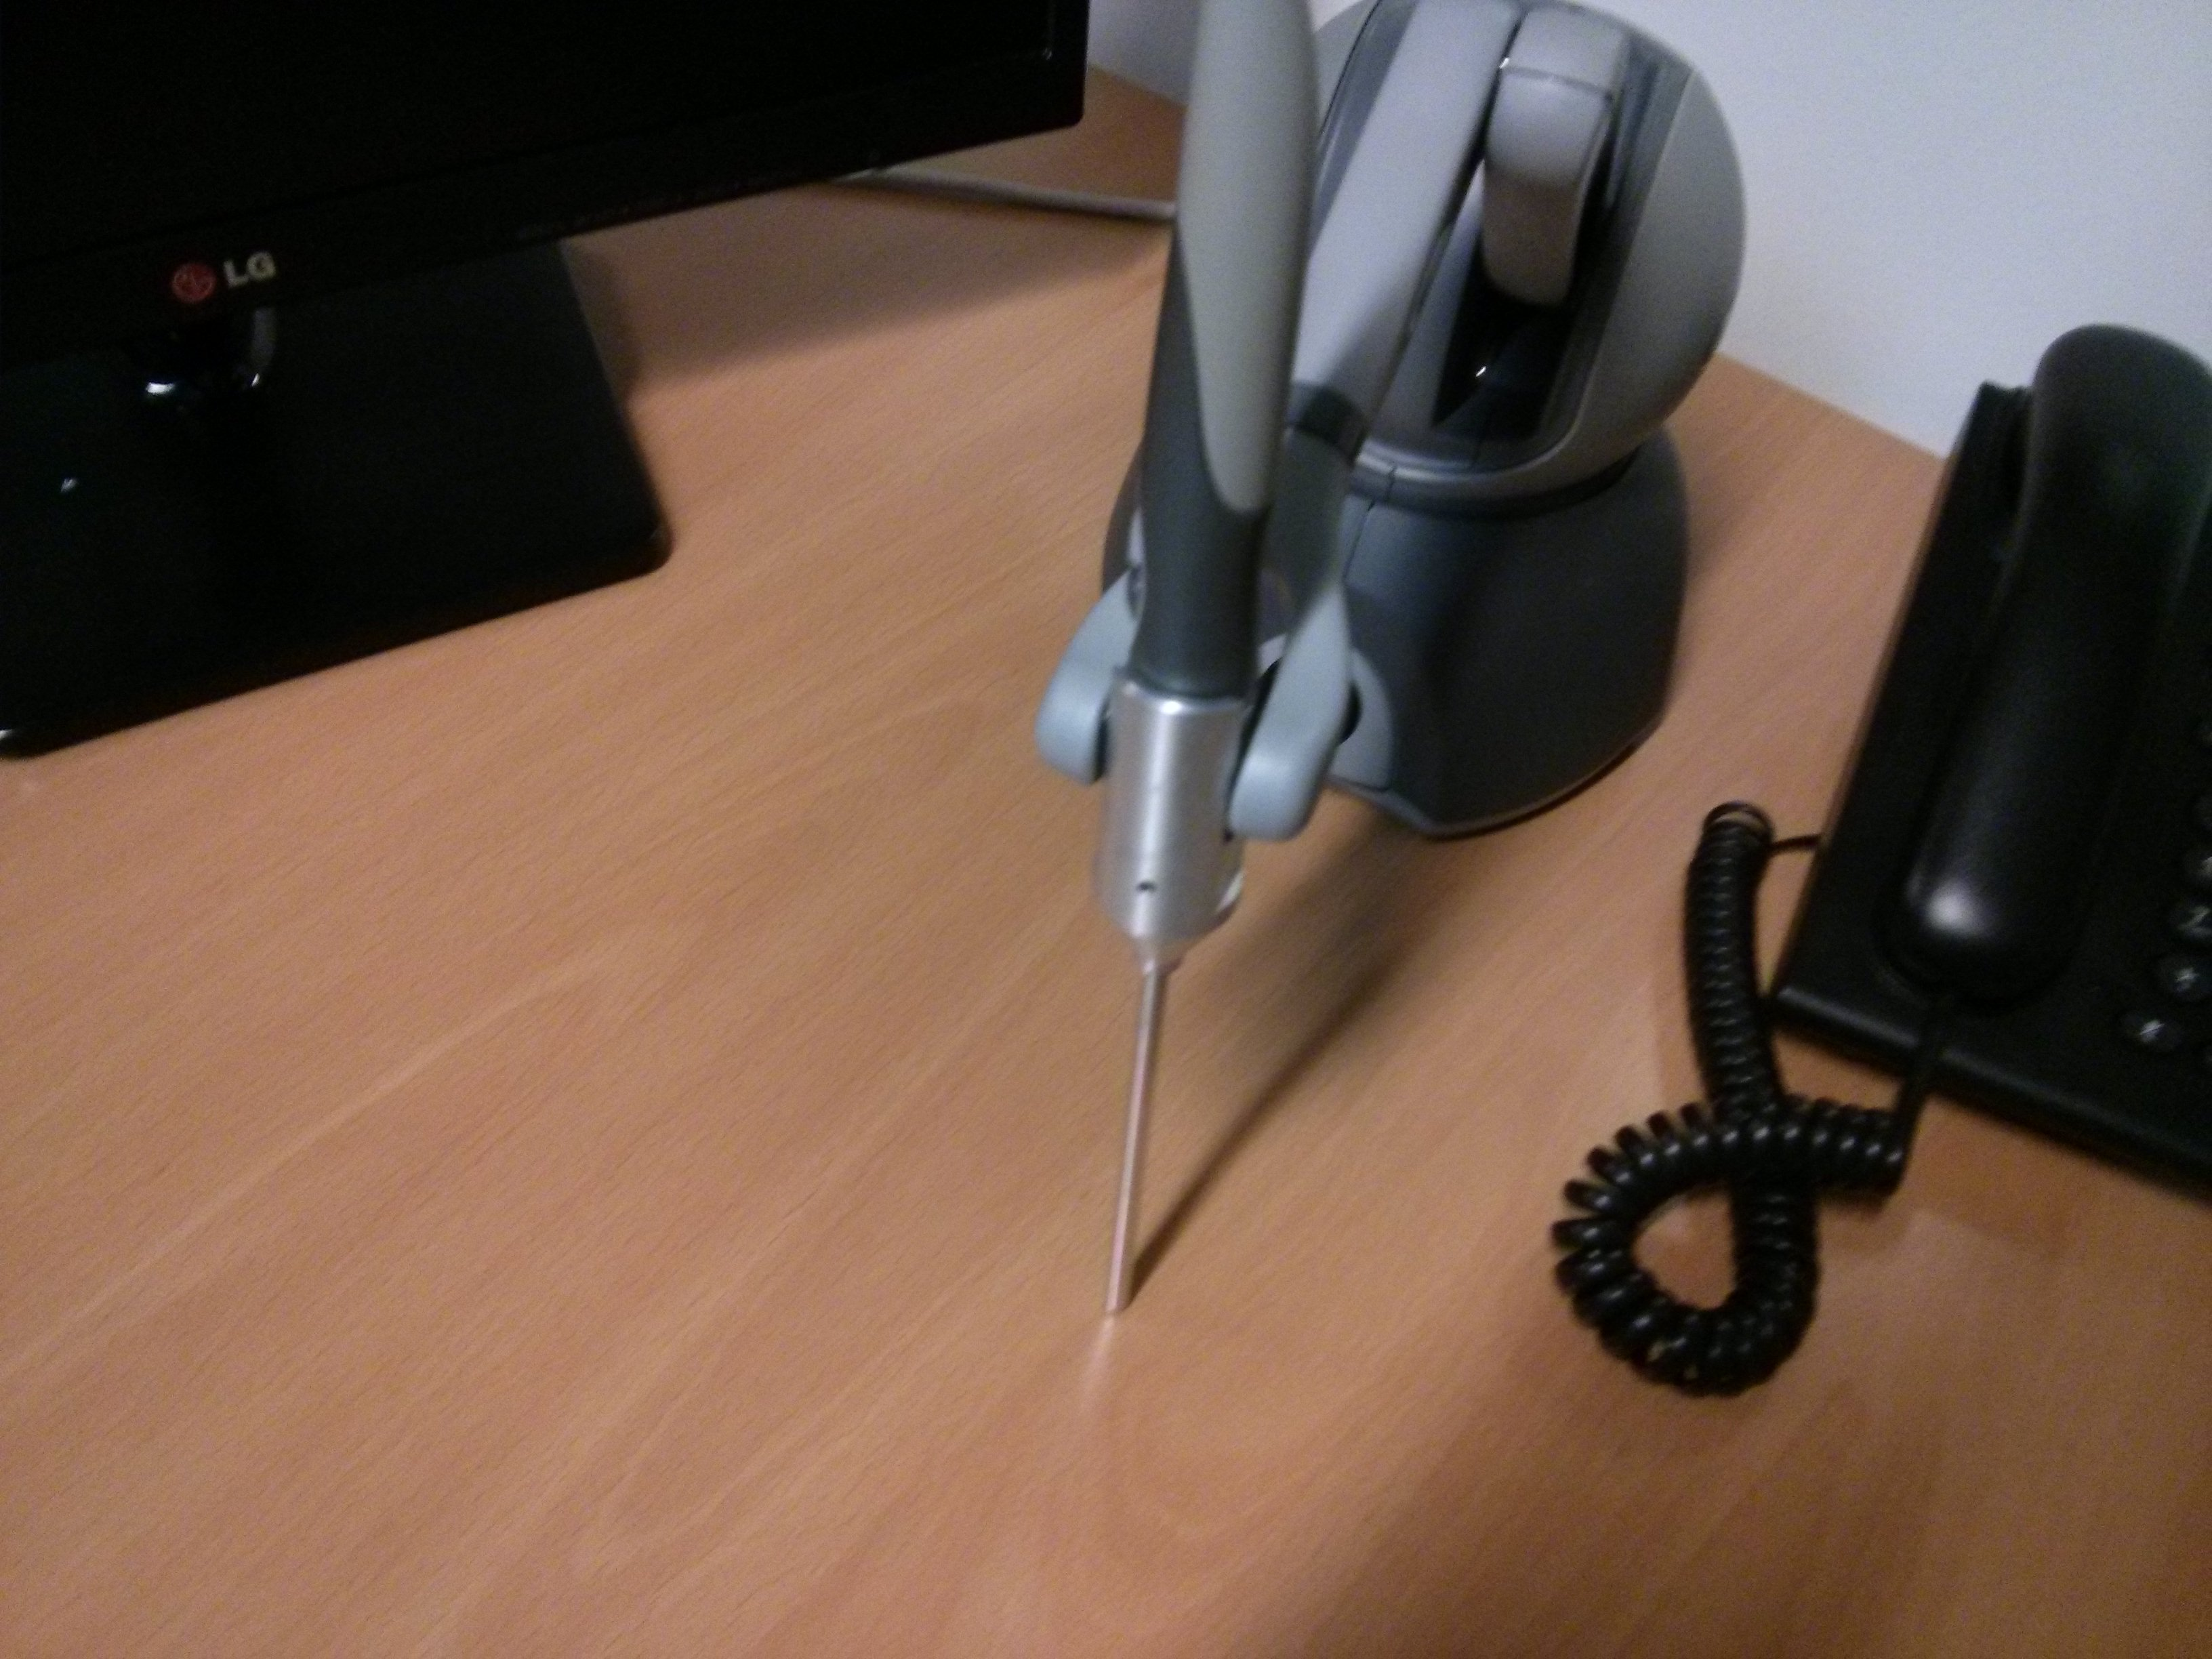
\includegraphics[width=0.5\textwidth]{IMG/needle2.jpg}
    \caption{Prototipo para permitir sujetar la aguja sin desplazamientos en el dispositivo háptico.}
    \label{fig:needle2}
\end{figure}
\todo{rehacer la imagen de la aguja}



Otro problema derivado de la selección del dispositivo era que el espacio de trabajo es limitado y cuanto más cerca se trabaja del límite de este espacio, más inestable puede ser el comportamiento del dispositivo. Afortunadamente el procedimiento de \ac{RA} tiene también un espacio limitado de acción y puede simplificarse la solución a este problema. Se propuso crear una mesa de trabajo que limite la acción del usuario al área de interés. 








\subsubsection{Mesa de trabajo}

El principal objetivo de crear una mesa de trabajo del simulador es estandarizar la posición relativa de los dispositivos anteriormente citados. Además de suplir las carencias de estos para mejorar la inmersión del usuario en el simulador.

Se ha diseñado una plataforma en forma de \emph{"T"}  para poder incorporar de manera perpendicular el campo de trabajo del dispositivo magnético por una parte y el dispositivo háptico por otra. Situando en el centro se colocará un maniquí de un material deformable para simular una zona anatómica del paciente. De esta manera, el dispositivo háptico puede ser intercambiado de posición para permitir que el simulador pueda ser configurado con el objetivo de que se pueda realizar con ambas manos. 
Los monitores estarán colocados de manera frontal para que el usuario tenga todos los elementos en el rango de visión y evitar la rotación de cuello. Una versión del prototipo se puede ver en la figura \ref{fig:simulator}.


\begin{figure}[h]
    \centering
    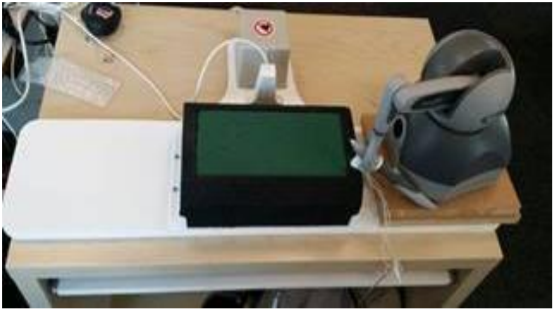
\includegraphics[width=0.5\textwidth]{IMG/simulator.PNG}
    \caption{Diseño de la mesa de trabajo con un rectángulo de espuma relleno de espuma floral. El emisor del dispositivo magnético está situado en el centro, el dispositivo háptico puede ser intercambiado de posición.}
    \label{fig:simulator}
\end{figure}


\paragraph{Maniquí} \mbox{}\\
En el procedimiento de \ac{RA}, el radiólogo apoya la sonda de ultrasonidos y parte del brazo en la anatomía del paciente. Por tanto, era necesario simular cierta zona que ayudará al usuario a apoyar la sonda de ultrasonidos e introducir la aguja en algún lugar de manera segura y controlada. Esto requería que el material fuera resistente tanto a presión como a la inserción de la aguja repetidamente sin introducir fuerzas adicionales al sistema. Se diseño un rectángulo de espuma de poliuretano que sirviera de recipiente para un relleno con espuma floral como se puede observar en la figura \ref{fig:simulator}.

La idea original era obtener un reemplazo rápido porque la espuma floral, aunque permitía una inserción de la aguja sin apenas resistencia, era muy débil ante presión y rotaciones de la aguja. Además, las inserciones continuas debilitaban el material y pueden dar información a los usuarios que utilicen el simulador posteriormente.
Para añadir consistencia a la espuma floral se ideó añadir una capa de silicona por encima. Esta capa permitía que la espuma no se deshiciera con el rozamiento y además proporcionaba cierta estabilidad, pero a la vez introducía un pequeño rozamiento que habría que salvar al introducir una aguja. En la figura \ref{fig:silicona} se puede observar un prototipo.

\begin{figure}[h]
    \centering
    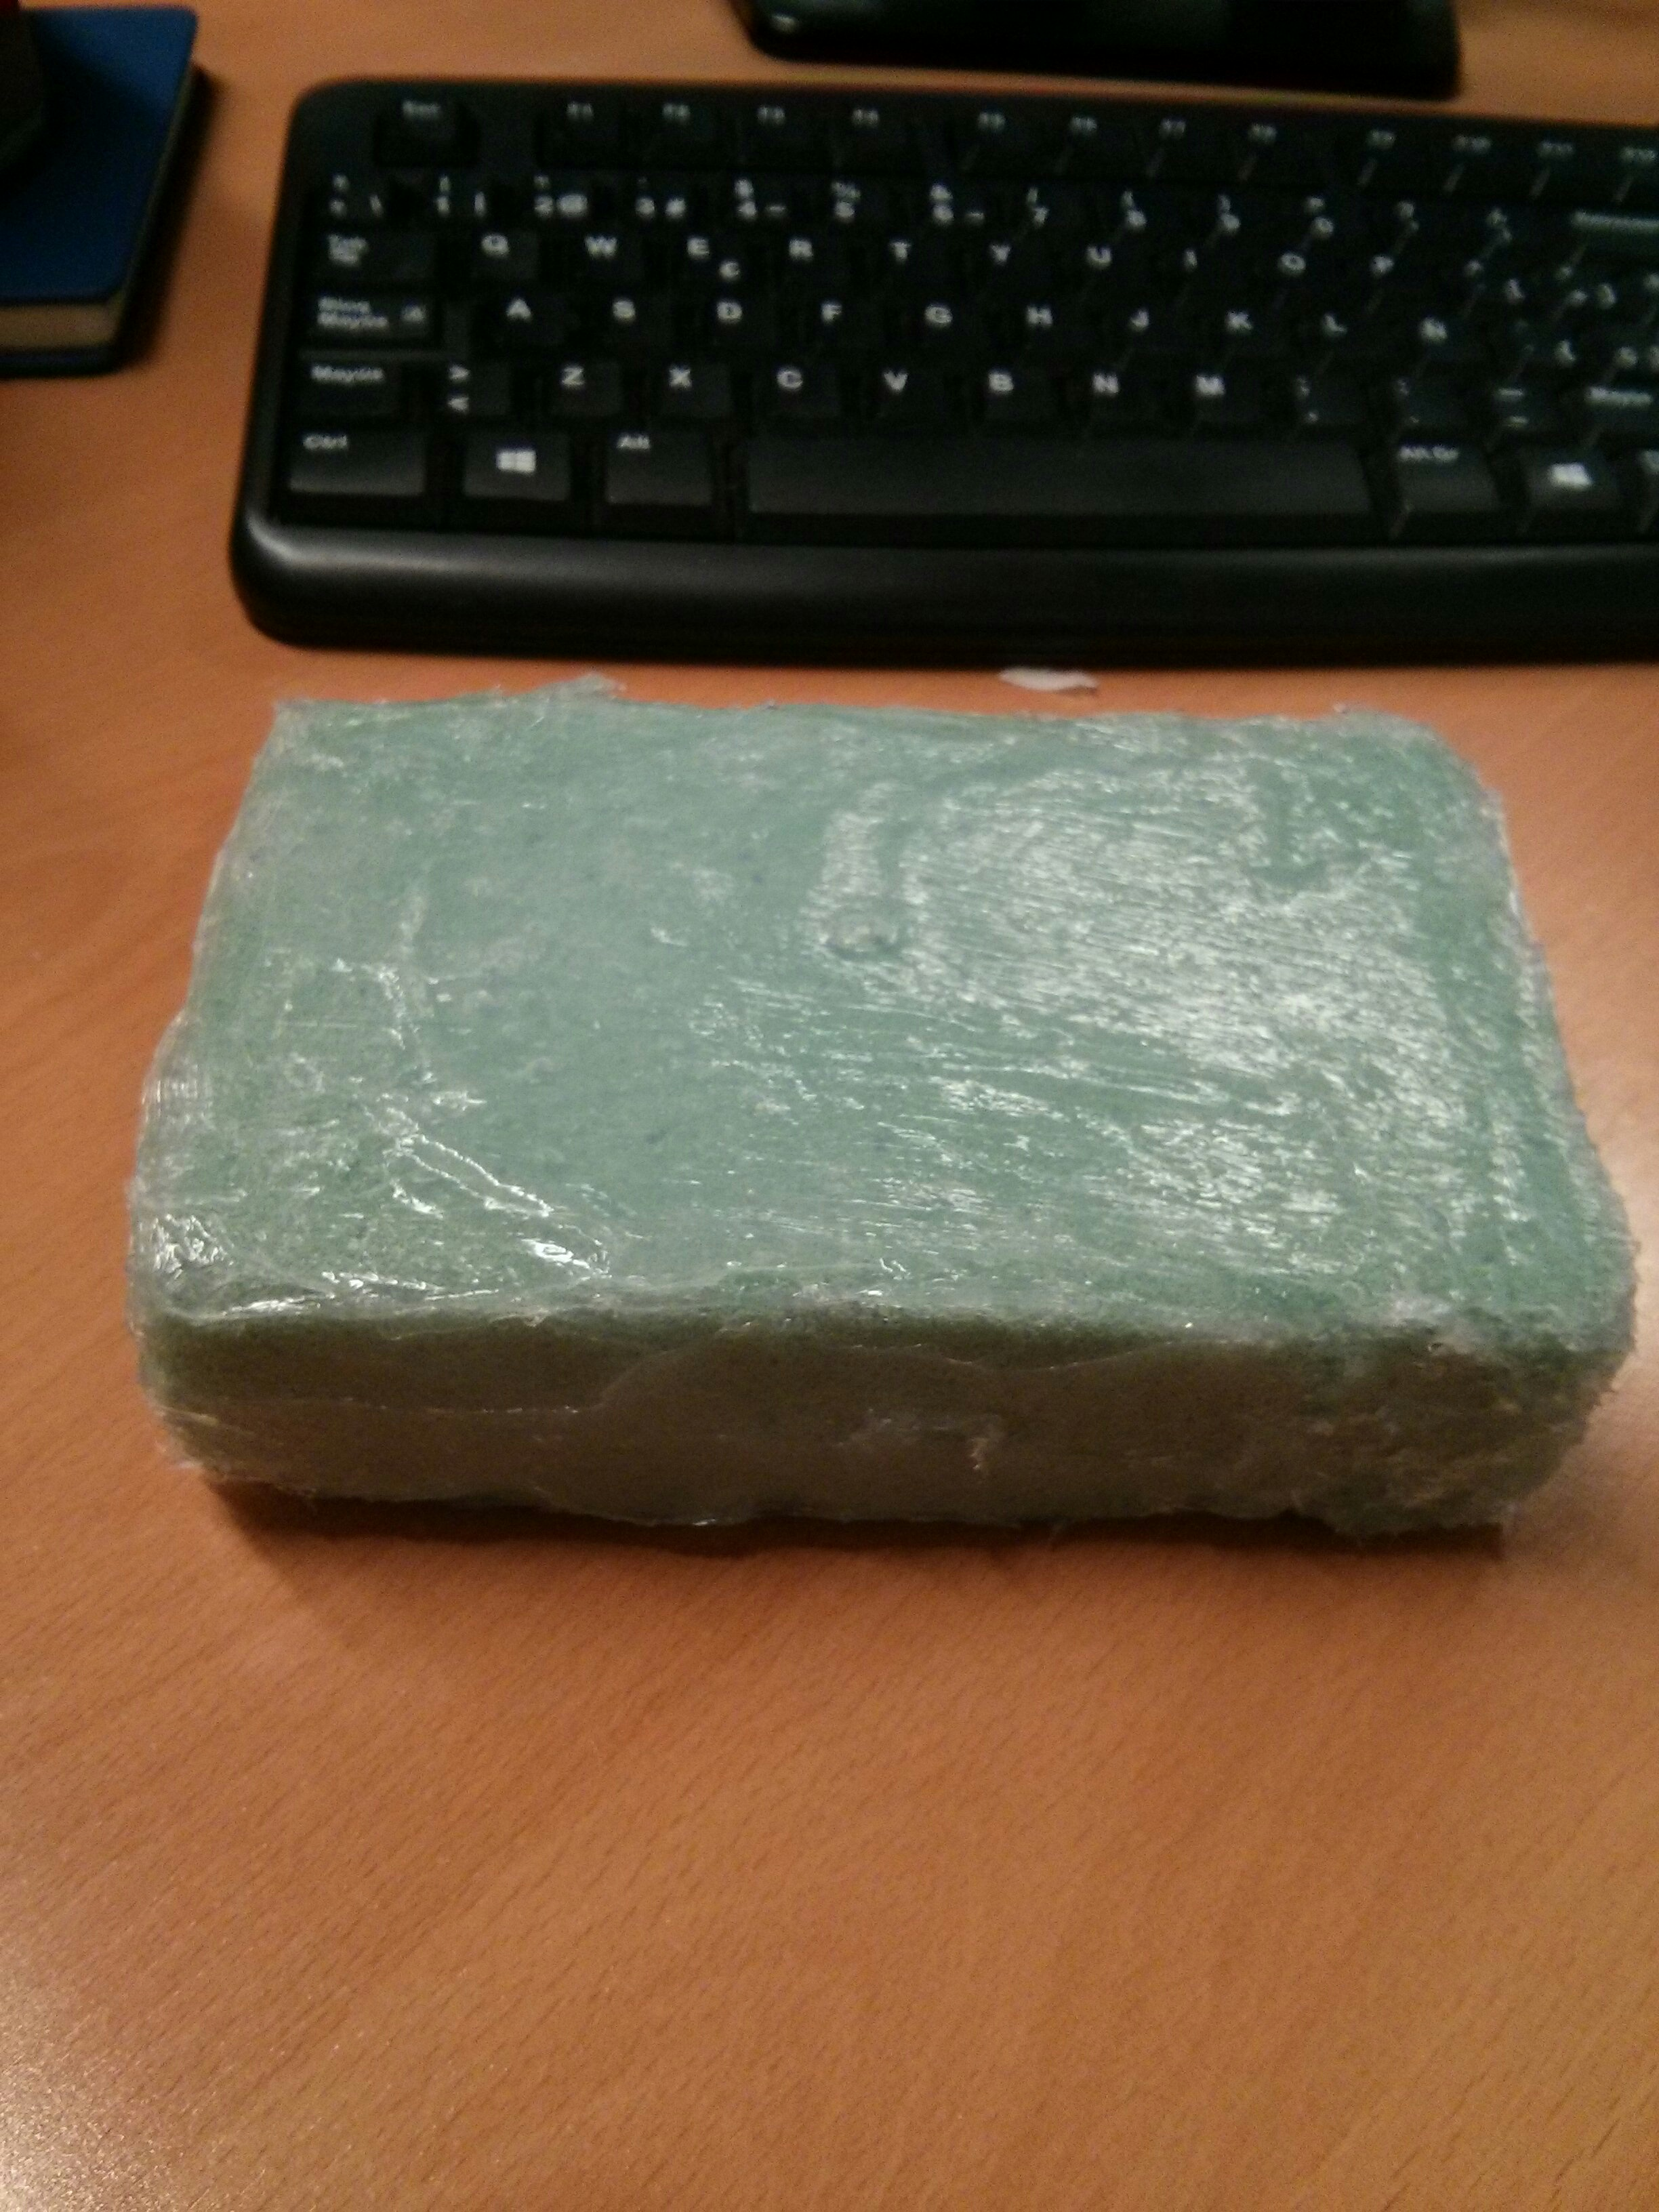
\includegraphics[width=0.5\textwidth]{IMG/silicona.jpg}
    \caption{Espuma floral cubierta de una capa de silicona para mejorar su consistencia.}
    \label{fig:silicona}
\end{figure}

Desde la \ac{URJC} se propuso utilizar otro material que no implique un bloque de espuma. Existe un material arenoso que intenta simular un fluido \emph{no newtoniano} (ver figura: \ref{fig:arena}) de tal forma que es resistente a la presión y rozamiento de la sonda, pero permite una inserción de la aguja sin apenas resistencia. Además, al ser un material con características parecidas a las de un fluido, las continuas inserciones no debilitan el material. Puede ser fácilmente reemplazable y su coste es pequeño.


\begin{figure}[h]
    \centering
    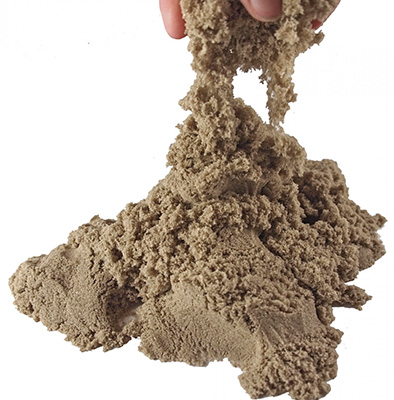
\includegraphics[width=0.5\textwidth]{IMG/arena.jpg}
    \caption{Arena \emph{kinética}}
    \label{fig:arena}
\end{figure}
\todo{rehacer figura arena}

Existen otros problemas al restringir el espacio de trabajo a un rectángulo de espuma o arena. Este rectángulo no representa fielmente el modelo anatómico. Al no ser iguales que el modelo del paciente virtual, esto generaba inconsistencias entre el mundo virtual y el real que afectaba a la realización correcta del procedimiento.
Actualmente, la tecnología de impresión 3D permite una solución rápida y barata para fabricar modelos personalizados. Con el objetivo de mejorar el realismo de la aplicación, se ha diseñado el rectángulo contenedor que tuviera la forma anatómica utilizando el mismo modelo que se usaría en el simulador. Solo haría falta introducir y adaptar la espuma o arena en el interior de este modelo. Esto permitiría utilizar la forma anatómica como se puede observar en la figura \ref{fig:pierna}. 

\begin{figure}[h]
    \centering
    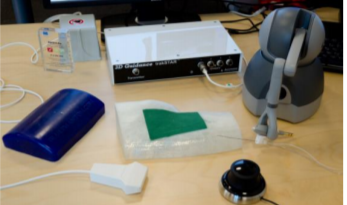
\includegraphics[width=0.5\textwidth]{IMG/pierna.PNG}
    \caption{Versión del contenedor de la espuma con forma de pierna.}
    \label{fig:pierna}
\end{figure}

Aun así, esta solución depende enormemente del modelo anatómico que se esta simulando y necesitaría imprimir un soporte para cada modelo virtual que se utilizará en el simulador. 


\subsubsection{Software}

Con el objetivo de mostrar la versatilidad y comprobar la hipótesis de esta tesis, se ha contribuido al proyecto \ac{RASimAs} con la generación de un módulo de entrenamiento que permita utilizar los modelos generados por el algoritmo de posicionamiento de pacientes virtuales. El desarrollo de este módulo y su posterior evaluación demostraría la capacidad del algoritmo propuesto en un ejemplo de caso de uso.

Tanto el motor de \ac{RV} como los dispositivos de entrada y salida no podrían ser capaces de servir como herramienta de aprendizaje por si mismos si no hubiera un software que guía las tareas y las acciones del usuario cuando utiliza el simulador.
El módulo de \ac{Courseware} es una pieza fundamental en \ac{RASim} ya que gestiona la comunicación entre componentes, ayuda y recopila información de los usuarios. Se encarga de recopilar información de los dispositivos y se comunica con la base de datos que almacena las métricas de los usuarios. A la vez, será la aplicación encargada de manejar las ventanas y la interacción del usuario con el sistema. 

El usuario podrá identificarse en el simulador a través de una interfaz. La aplicación recibirá el perfil desde el servidor y basándose en el perfil del usuario, el \ac{Courseware} proporcionara el escenario de entrenamiento según el protocolo que se haya definido. Incluso este módulo es el encargado de descargar nuevos escenarios del simulador desde el servidor. 

Debido a la complejidad e importancia de este módulo, será descrito en una sección independiente a continuación.

